\documentclass{article}

\usepackage[polish]{babel}
\usepackage[utf8]{inputenc}
\usepackage{polski}
\usepackage[T1]{fontenc}
\usepackage{url}
\usepackage{xcolor}
\usepackage{listings} %for shell commands listing
\frenchspacing
\usepackage{indentfirst}
\usepackage{graphicx}

\addtolength{\textwidth}{3cm}
\addtolength{\hoffset}{-1.5cm}
\addtolength{\textheight}{3cm}
\addtolength{\voffset}{-1.5cm}

\lstdefinestyle{bash}{
  language=bash,
  basicstyle=\small\sffamily,
  stringstyle=\ttfamily, % typewriter type for strings
  numbers=none,
  numberstyle=\tiny,
  numbersep=3pt,
  showstringspaces=false, % no special characters instead of spaces
  keywordstyle=,%\color{black}\bfseries, %keywords in bold
  frame=tb,
  columns=fullflexible,
  backgroundcolor=\color{gray!20},
  linewidth=1.0\linewidth,
  xleftmargin=0.0\linewidth
}

\begin{document}

\title{Apache Cassandra 2.0\\\vspace{2ex}Przewodnik instalacji i konfiguracji w systemie Debian Wheezy}
\author{Jan Baranowski, Michał Kaik\\Politechnika Poznańska}
\maketitle

\section{Wstęp}

Niniejszy dokument ma za zadanie przedstawić proces instalacji i konfiguracji serwera baz danych NoSQL \emph{Apache Cassandra} w środowisku rozproszonym.
Na potrzeby demonstracji zakłada się że środowisko to będzie składać się z kilku węzłów połączonych siecią lokalną.

Apache Cassandra jest serwerem baz danych NoSQL, początkowo rozwijanym przez Facebooka na potrzeby umożliwienia efektywnego przeszukiwania skrzynki odbiorczej. Obecnie Cassandra jest rozwijana przez Apache Foundation (jest jednym z projektów top-level) i stanowi podstawę dla zestawu narzędzi DataStax. 

Cassandra powstała jako narzędzie mające w założeniu cechować się:
\begin{itemize}
\item wysoką dostępnością (Cassandra jest określana jako zawsze zapisywalna baza danych)
\item niskim opóźnieniem wykonywanych operacji (ang. latency)
\item odpornością na awarie (możliwością replikacji danych, brakiem komponentów, których awaria może zdestabilizować system (ang. single points of failure))
\item możliwością regulacji kompromisu pomiędzy szybkością działania a odpornością na awarie i spójnością replik
\item relatywnie prostym modelem danych
\end{itemize}

Zarówno opisanie kolumnowego modelu danych wykorzystywanego w Cassandrze, jak i mechanizmów, dzięki którym spełnia ona założenia projektowe nie jest celem tego dokumentu. Autorzy mogą jedynie podać propozycje publikacji, które opisują wspomniane zagadnienia. Zarówno dla modelu danych, jak i budowy wewnętrznej Cassandry będzie to przede wszystkim dokumentacja udostępniana przez firmę DataStax ([link]). Model danych, przedstawiony z perspektywy osób pracujących z bazami relacyjnymi został doskonale (choć może zbyt obszernie) opisany w Cassandra - The Definitive Guide ([x]). Z kolei architektura Cassandry w dużym skrócie (choć zapewne w sposób wystarczający by służyć jako wstęp do tego dokumentu) została przedstawiona w prezentacji \cite{JanBaranowski2014}.

Procedurę przygotowania klastra przedstawiono na przykładzie systemu operacyjnego Debian GNU/Linux 6, ponieważ uchodzi on za jedno z lepszych rozwiązań dla serwerów.

\section{Wybór dystrybucji}

Na początku nowi użytkownicy Cassandry stają przed wyborem dystrybucji tego oprogramowania. Możliwości są dwie: instalacja standardowej wersji Cassandry, dostarczonej przez Apache Foundation oraz instalacja platformy DataStax - zestawu narzędzi obudowujących Cassandrę i dostarczających m.in. funkcje pozwalające na uproszczenie zarządzania klastrem, monitorowanie przy użyciu narzędzi wizualnych, analizę obciążeń węzłów, itp. (por. Rysunek \ref{datastax_arch}).

\begin{figure}[h]
\centering
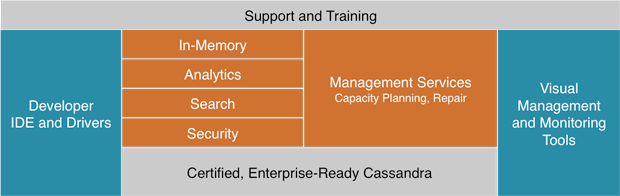
\includegraphics[width=\linewidth]{gfx/datastax}
\caption{architektura DataStax w odniesieniu do Cassandry, źródło: \cite{whydatastax}}
\label{datastax_arch}
\end{figure}

Wybór jest ważny o tyle, że pomimo wspólnego fundamentu, jakim jest Cassandra, procesy instalacji obu dystrybucji nie mają ze sobą nic wspólnego, tj. (według wiedzy autorów) nie da się doinstalować do dystrybucji Apache platformy DataStax.

W tym miejscu należy wspomnieć o twórcach platformy -- firmie o zaskakującej nazwie DataStax, zajmującej się dostosowaniem Cassandry do potrzeb przedsiębiorstw poprzez m.in. rozwój i testowanie Cassandry, dostarczanie narzędzi ułatwiających administrację systemem, organizację szkoleń, certyfikację personelu technicznego, itd. Bodaj najbardziej znaczącym wkładem DataStax w rozwój projektu jest opracowanie szeregu konektorów dla różnych języków programowania, dzięki którym programiści mogą korzystać z bazy danych w sposób analogiczny do rozwiązań relacyjnych (np. tak jak w przypadku MySQL Connectors, por. \cite{mysql_connectors}) i rozbudowa dokumentacji technicznej platformy, włączając w to dokumentację plików konfiguracyjnych, architektury Cassandry i języka CQL (odpowiednika SQL dla kolumnowych baz danych, których przedstawicielem jest Cassandra).

Na potrzeby niniejszego dokumentu założono, że właściwym wyborem będzie dystrybucja Apache Cassandra, ze względu na to, że dokument ma pełnić rolę wprowadzenia do technologii, nie zaś pozwalać na błyskawiczne wdrożenie systemu (ang. rapid deployment). Poza tym, przewodniki instalacji i konfiguracji DataStaxa dostępne są np. na stronie \cite{datastax_guides}.

\section{Instalacja}

Cassandra zostanie zainstalowana przy użyciu narzędzia APT z repozytorium Apache Software Foundation. Wymagane będzie dodanie odpowiedniego repozytorium do listy źródeł APTa. Dodatkowo ze względu na to, że Cassandra napisana jest w Javie, pokazany zostanie proces instalacji Oracle JVM w systemie Debian (ta maszyna wirtualna jest zalecana przez twórców Cassandry).

\subsection{Wybór maszyny wirtualnej Java}

Apache Software Foundation dostarcza pakiety zawierające Cassandrę w formacie *.deb, a także repozytorium dla APTa. Jedną z zależności pakietu "cassandra" jest pakiet "openjdk-7-jre". Jest to w pewnym sensie sprzeczne z zaleceniami twórców Cassandry, ponieważ ci rekomendują maszynę wirtualną Oracle jako środowisko uruchomieniowe (nawet w testowanej wersji 2.0 bazy danych odpowiedni komunikat wyświetlany jest w logu). Nie zmienia to faktu, że testy (funkcjonalne, lecz nie wydajnościowe) przeprowadzone na potrzeby stworzenia tego artykułu udowodniły, że Cassandra działa bez zarzutu także w środowisku OpenJDK. 

Należy zatem wybrać pomiędzy stosowaniem się do zaleceń a prostotą instalacji.

\subsection{Instalacja i konfiguracja Oracje Java}

Pakiet z OpenJDK jest instalowany jako pakiet zależny podczas instalacji Cassandry. Jeżeli jednak administrator zdecyduje się użyć Oracle JVM, poniżej przedstawiona jest skrótowa procedura instalacji tego oprogramowania w systemie Debian. Stanowi ona kompilację najprostszych rozwiązań i tym różni się od większości przewodników dostępnych w internecie, że poza konsolą systemu nie wymaga żadnych dodatkowych narzędzi (np. mechanizmu transferu plików z maszyny-terminala do maszyny-serwera).

Pierwszym krokiem jest pobranie pakietu oprogramowania (JRE, nie JDK) ze strony Oracle. Standardowo by pobrać plik należy zaakceptować umowę licencyjną Oracle, jednak przy odpowiedniej konfiguracji możliwe jest ominięcie tego kroku \cite{downloading_oracle_java}:

\begin{lstlisting}[style=bash, caption={pobieranie Oracle JRE}]
$ wget --no-cookies \
> --no-check-certificate \
> --header "Cookie: oraclelicense=accept-securebackup-cookie" \
> "http://download.oracle.com/otn-pub/java/jdk/7u60-b19/jre-7u60-linux-i586.tar.gz" \
> -O /tmp/jre-7u60-linux-i586.tar.gz
\end{lstlisting}

Popularnym sposobem instalacji pobranego oprogramowania jest wypakowanie archiwum (zazwyczaj do katalogu /opt) i ręczna konfiguracja ścieżki systemowej (por. \cite{downloading_oracle_java}). Debian dostarcza jednak narzędzie pozwalające przekonwertować archiwum do pakietu DEB \cite{installing_oracle_java_on_debian}.

Należy je zainstalować, a potem użyć:

\begin{lstlisting}[style=bash, caption={budowa pakietu DEB z Oracle JRE}]
$ apt-get install java-package

$ fakeroot make-jpkg /tmp/jre-7u60-linux-i586.tar.gz
\end{lstlisting}

Powstały w ten sposób pakiet należy zainstalować. Po instalacji należy ustawić Oracle JVM jako domyślną maszynę wirtualną w systemie.

\begin{lstlisting}[style=bash, caption={instalacja i konfiguracja Oracle JRE}]
$ dpkg -i /tmp/oracle-j2re1.7\textunderscore 1.7.0+update60_i386.deb

$ update-alternatives --config java
There are 2 choices for the alternative java (providing /usr/bin/java).

  Selection    Path                                           Priority   Status
------------------------------------------------------------
  0            /usr/lib/jvm/java-7-openjdk-i386/jre/bin/java   1051      auto mode
* 1            /usr/lib/jvm/j2re1.7-oracle/bin/java            316       manual mode
  2            /usr/lib/jvm/java-7-openjdk-i386/jre/bin/java   1051      manual mode

Press enter to keep the current choice[*], or type selection number:

$ java -version
java version "1.7.0_60"
Java(TM) SE Runtime Environment (build 1.7.0_60-b19)
Java HotSpot(TM) Client VM (build 24.60-b09, mixed mode)
\end{lstlisting}

Według wiedzy autorów Cassandra nie wymaga ustawiania zmiennej \lstinline[style=bash]!JAVA_HOME! dla żadnego z użytkowników (ani roota, ani użytkownika \textit{cassandra}, właściciela demona). Jeżeli jednak zajdzie taka potrzeba, zainstalowane maszyny wirtualne można znaleźć w katalogu /usr/lib/jvm.

\begin{lstlisting}[style=bash, caption={ustawianie JAVA\textunderscore HOME}]
$ echo "export JAVA_HOME=/usr/lib/jvm/j2re1.7-oracle/" >> /home/<user>/.bashrc
\end{lstlisting}

\subsection{Konfiguracja repozytorium}

By móc zainstalować Cassandrę, należy dodać odpowiednie repozytorium Apache Software Foundation do źródeł programu APT. Zgodnie z konwencją każda większa wersja Cassandry znajduje się w osobnym repozytorium. Na potrzeby tego dokumentu zostanie zainstalowana Cassandra 2.0.8.

Do pliku \lstinline[style=bash]!/etc/apt/sources.list! należy dopisać:

\begin{lstlisting}[style=bash, caption={nowe źródłą pakietów dla APTa}]
deb http://www.apache.org/dist/cassandra/debian 20x main
deb-src http://www.apache.org/dist/cassandra/debian 20x main
\end{lstlisting}

Próba pobrania spisu zawartości repozytorium zakończy się niepowodzeniem, ponieważ APT nie zna kluczy publicznych dla repozytorium Apache SF. Te należy dodać w następujący sposób:

\begin{lstlisting}[style=bash, caption={pobieranie kluczy publicznych repozytorium ASF}]
$ gpg --keyserver pgp.mit.edu --recv-keys F758CE318D77295D
$ gpg --export --armor F758CE318D77295D | sudo apt-key add -

$ gpg --keyserver pgp.mit.edu --recv-keys 2B5C1B00
$ gpg --export --armor 2B5C1B00 | sudo apt-key add -
\end{lstlisting}

Po zakończeniu wszystkich operacji należy pobrać spis zawartości repozytoriów:
\begin{lstlisting}[style=bash, caption={odświeżanie list pakietów}]
$ apt-get update
\end{lstlisting}

\subsection{Instalacja Cassandry}

Ostatnim krokiem procesu instalacji jest zainstalowanie Cassandry z użyciem APTa:
\begin{lstlisting}[style=bash, caption={instalacja Cassandry}]
$ apt-get install cassandra
\end{lstlisting}

W efekcie Cassandra powinna zostać zainstalowana i uruchomiona.

\section{Konfiguracja węzła}

Ta część dokumentu opisuje czynności związane z konfiguracją węzła Cassandry tak, by był on zdolny dołączyć do klastra. Cassandra jest systemem P2P, więc o utworzeniu klastra węzły decydują wspólnie w oparciu o taką samą nazwę klastra zdefiniowaną w pliku konfiguracyjnym i włączony kanał komunikacji poprzez plotkowanie. Kanał ten jest domyślnie wyłączony, zatem każdy węzeł Cassandry w sieci będzie z początku tworzył osobny klaster.

\subsection{Stan systemu po instalacji}\label{system_state}

Zaraz po instalacji w systemie pojawia się nowa usługa: cassandra. Jest ona domyślnie uruchomiona. Jej konfiguracja zapobiega możliwości dołączenia węzła do jakiegokolwiek klastra ze względu na zablokowanie mechanizmu plotkowania (dokładnie: agent implementujący algorytm plotkujący nasłuchuje na adresie IP 127.0.0.1).

Pliki konfiguracyjne można znaleźć w katalogu \lstinline[style=bash]!/etc/cassandra!. Są wśród nich:
\begin{itemize}
\item \lstinline[style=bash]!/etc/cassandra/cassandra-env.sh! - skrypt definiujący zmienne środowiskowe w formie argumentów dla maszyny wirtualnej Java (np. wielkość stosu, ale także: włączenie/wyłączenie mechanizmu JMX)
\item \lstinline[style=bash]!/etc/cassandra/cassandra-rackdc.properties! - informacja o tym, w którym fizycznie racku i centrum danych znajduje się obecny węzeł
\item \lstinline[style=bash]!/etc/cassandra/cassandra-topology.properties! - przybliżone informacje o tym, w których rackach i centrach danych znajdują się inne węzły klastra. Plik ten jest wykorzystywany przez jedną z kilku wersji algorytmu rozmieszczania replik
\item \lstinline[style=bash]!/etc/cassandra/cassandra-topology.yaml! - plik analogiczny do poprzedniego, wykorzystywany jednak przez inną wersję algorytmu
\item \lstinline[style=bash]!/etc/cassandra/cassandra.yaml! - główny plik konfiguracyjny Cassandry
\end{itemize}

Pliki danych (w tym: commit logi) znaleźć można w katalogu \lstinline[style=bash]!/var/lib/cassandra!. Czyszcząc zawartość 3 znajdujących się w nim podkatalogów można zresetować stan klastra. W celu wykonania tej czynności autorzy nie zalecają jednak ich usuwania (podczas testowania mogą one zostać utworzone na nowo z prawem zapisu tylko dla roota, co uniemożliwi normalny start usługi).

Plik logu znaleźć można w \lstinline[style=bash]!/var/log/cassandra/system.log!

\subsection{Jak debugować konfigurację?}

Przed rozpoczęciem wprowadzania zmian do plików konfiguracyjnych zaleca się wyłączenie automatycznego uruchamiania usługi. Błędnie skonfigurowany węzeł może dołączyć do nieodpowiedniego klastra, a jego usunięcie w takim przypadku nie jest zadaniem trywialnym. Efekt można osiągnąć wykonując polecenie:

\begin{lstlisting}[style=bash, caption={wyłączenie uruchamiania Cassandry na jej domyślnych runlevelach}]
$ insserv -r cassandra
\end{lstlisting}

Najprostszym sposobem sprawdzenia poprawności konfiguracji jest uruchomienie węzła w trybie jawnym (w przeciwieństwie do deamona). Służy do tego podane poniżej polecenie, które wypisze log działania węzła na standardowe wyjście.

\begin{lstlisting}[style=bash, caption={wyłączenie uruchamiania Cassandry na jej domyślnych runlevelach}]
$ cassandra -f  # -f for foreground
\end{lstlisting}

Dodatkowo można zarchiwizować taki log poleceniem \lstinline[style=bash]!tee plik.log!, które skopiuje standardowe wejście na standardowe wyjście i do podanego pliku:

\begin{lstlisting}[style=bash, caption={wyłączenie uruchamiania Cassandry na jej domyślnych runlevelach}]
$ cassandra -f | tee /tmp/cassandra_testrun.log
\end{lstlisting}

\textbf{UWAGA!} Jeżeli Cassandra zostanie uruchomiona w trybie jawnym podczas gdy równolegle usługa działa w tle, zamiast informacji o błędzie w logu tej pierwszej pojawi się informacja o wyjątku NullPointerException.

\textbf{UWAGA!} Jeżeli pierwsze uruchomienie Cassandry odbędzie się w trybie jawnym z poziomu użytkownika innego niż "cassandra", usługa nie będzie miała prawa zapisu do katalogów danych, nie będzie więc w stanie się uruchomić.

\textbf{UWAGA!} Jeżeli zmienna \lstinline[style=bash]!JAVA_HOME! dla użytkownika uruchamiającego polecenie \lstinline[style=bash]!cassandra -f! jest ustawiona, ale prowadzi do poprawnie zainstalowanej maszyny wirtualnej, cassandra nie uruchomi się, ale ani skrypt startowy ani log nie poinformują o błędzie.

\pagebreak

\subsection{Pliki konfiguracyjne}

Role podstawowych plików konfiguracyjnych zostały przedstawione w punkcie \ref{system_state}. Tutaj (w tabeli \ref{config_table}) zostaną opisane parametry konfiguracyjne (z \lstinline[style=bash]!/etc/cassandra/cassandra.yaml!), których wartości powinny zostać świadomie dobrane przed uruchomieniem pojedynczego węzła.

Konfigurację węzła ułatwia główny plik konfiguracyjny Cassandry, zawierający obszerne komentarze.

\begin{table}[hhh]
\caption{podstawowe parametry konfiguracyjne Cassandry (w \lstinline[style=bash]!/etc/cassandra/cassandra.yaml!).}
\label{config_table}
\begin{tabular}{|r|c|p{8cm}|}
\hline 
\textbf{Parametr} & \textbf{Linia} & \textbf{Komentarz}\\
\hline
\hline
cluster\_name & 10 & nazwa klastra, którego ten węzeł jest członkiem\\
\hline
seed\_provider/parameters/seeds & 192 & węzeł Cassandry nie odkrywa innych węzłów automatycznie, stąd dla algorytmu plotkowania wymagana jest lista początkowych "punktów kontaktowych". Oczywiście punkty powinny być tak dobrane by nie dopuścić do partycjonowania klastra.\\
\hline
listen\_address & 297 & adres IP kanału komunikacyjnego pomiędzy węzłami. Agent algorytmu plotkującego będzie nasłuchiwał na tym adresie. Jeżeli wartość nie zostanie tutaj podana, Cassandra wybierze adres IP local hosta.\\
\hline
start\_rpc & 324 & czy uruchomić serwer Thrift RPC. Wyłączenie serwera RPC uniemożliwi dostęp do węzła przez np. cqlsh.\\
\hline
rpc\_address & 335 & adres IP na którym ma nasłuchiwać serwer Thifta\\
\hline
\end{tabular} 
\end{table}

\subsection{Weryfikacja stanu węzła}

Szeroko pojęty stan węzła po konfiguracji można sprawdzić na kilka sposobów. Przede wszystkim po uruchomieniu usługi należy sprawdzić czy ta faktycznie działa i gdy tak nie jest, przejrzeć log.

W następnej kolejności można sprawdzić czy Cassandra nasłuchuje na portach zdefiniowanych w pliku konfiguracyjnym:

\begin{lstlisting}[style=bash, caption={sprawdzanie na których portach nasłuchuje Cassandra}]
$ netstat -ln4p  #listening, IPv4, numeric, with owner process information
\end{lstlisting}

Kolejnym sposobem jest próba połączenia się z węzłem poprzez Thrift API.
\begin{lstlisting}[style=bash, caption={dostęp do Cassandry przez Thrift API.}]
$ cqlsh localhost 9160 #use "quit;" to exit CQL shell
\end{lstlisting}

Wreszcie można wyświetlić stan klastra, do którego należy węzeł:
\begin{lstlisting}[style=bash, caption={sprawdzanie stanu klastra}]
$ nodetool --host localhost -p 7199 status # 7199 is the JMX port
Datacenter: datacenter1
=======================
Status=Up/Down
|/ State=Normal/Leaving/Joining/Moving
--  Address    Load       Tokens  Owns (effective)  Host ID                               Rack
UN  127.0.0.1  98.76 KB   256     100.0%            d85efd66-29fb-46d7-b824-a4cc3fc4e75b  rack1
\end{lstlisting}

\section{Konfiguracja klastra}

\subsection{Łączenie węzłów w klaster}

\subsection{Weryfikacja konfiguracji klastra}

\subsection{Działania dodatkowe}

\subsubsection{Synchronizacja zegarów}

\subsubsection{Czyszczenie}

\subsubsection{Konfiguracja uwierzytelniania}

\section{Zarządzanie klastrem}

\subsection{Monitoring węzłów i klastra}

\subsection{Przyłączanie i odłączanie węzłów}

\subsection{Backup danych}


\begin{thebibliography}{Xxx99x}

\bibitem[2]{mysql_connectors}
MySQL Connectors\\
\url{http://www.mysql.com/products/connector/}\\
dostęp 16 czerwca 2014 r.

\bibitem[3]{datastax_guides}
NoSQL Apache Cassandra Documentation\\
\url{http://planetcassandra.org/documentation/}\\
dostęp 16 czerwca 2014 r.

\bibitem[4]{downloading_oracle_java}
Daniel Stavrovski, Installing Oracle JAVA 7 on Debian Wheezy\\
\url{http://d.stavrovski.net/blog/post/installing-oracle-java-7-on-debian-wheezy}\\
dostęp 16 czerwca 2014 r.

\bibitem[5]{installing_oracle_java_on_debian}
Java/Sun, Debian Wiki\\
\url{https://wiki.debian.org/Java/Sun}\\
dostęp 16 czerwca 2014 r.

\bibitem[6]{whydatastax}
Why DataStax?\\
\url{http://www.datastax.com/why-datastax}\\
dostęp 16 czerwca 2014 r.

\end{thebibliography}

\end{document}